\documentclass[review]{elsarticle}

\usepackage{lineno,hyperref}
\modulolinenumbers[5]

\journal{Nuclear Instruments and Methods B}

%%%%%%%%%%%%%%%%%%%%%%%
%% Elsevier bibliography styles
%%%%%%%%%%%%%%%%%%%%%%%
%% To change the style, put a % in front of the second line of the current style and
%% remove the % from the second line of the style you would like to use.
%%%%%%%%%%%%%%%%%%%%%%%

%% Numbered
%\bibliographystyle{model1-num-names}

%% Numbered without titles
%\bibliographystyle{model1a-num-names}

%% Harvard
%\bibliographystyle{model2-names.bst}\biboptions{authoryear}

%% Vancouver numbered
%\usepackage{numcompress}\bibliographystyle{model3-num-names}

%% Vancouver name/year
%\usepackage{numcompress}\bibliographystyle{model4-names}\biboptions{authoryear}

%% APA style
%\bibliographystyle{model5-names}\biboptions{authoryear}

%% AMA style
%\usepackage{numcompress}\bibliographystyle{model6-num-names}

%% `Elsevier LaTeX' style
\bibliographystyle{elsarticle-num}
%%%%%%%%%%%%%%%%%%%%%%%

\begin{document}

\begin{frontmatter}

\title{Fluorescence yield for plastic scintillators after irradiation }


%% or include affiliations in footnotes:
\author[umd]{Zishuo Yang\corref{mycorrespondingauthor}}
\cortext[mycorrespondingauthor]{Corresponding author}
\ead{yangzs@terpmail.umd.edu}
\author[umd]{Alberto Belloni}
\author[umd]{Sarah C. Eno}
\author[eljen]{Charles Hurlbut}
\author[umd]{Kevin Pedro}
\author[umd]{Geng Yuan Jeng}
\author[umd]{Yao Yao}




\address[umd]{Dept. Physics, U. Maryland, College Park MD 30742 USA}
\address[eljen]{Eljen Technology, 1300 W. Broadway, Sweetwater, Tx 79556 USA}


\begin{abstract}
The ratio of the fluorescence yield versus wavelength for plastic scintillators EJ-408 and EJ-260 before and after irradiation by a $\rm {^{60}Co}$ source for doses of 50, 30, 10, 4, and 2 Mrad at various dose rates and for different concentrations of the primary and secondary dopant.  While the nominal dopant concentration gives the highest light output prior to irradiation, a higher concentration is found to be optimal for irradiated plastics.
\end{abstract}

\begin{keyword}
plastic scintillator\sep fluorescence\sep radiation hardness
\end{keyword}

\end{frontmatter}

\linenumbers

\section{Introduction}
Organic scintillators (such as toluene, polystyrene, and naphthalene) containing wave-length shifting
additives in solution have long been popular elements in detectors used
in particle physics, nuclear physics, radiation safety, and heath physics applications  due to their high light output, low cost, fast response,
and versatility of physical construction. 
Prolonged exposure of plastic scintillator to
ionizing radiation, however, can result in damage:
light self-absorption (yellowing) increases and 
initial light yield decreases.  
In this paper, we present measurements of ratio of the light output before and after irradiation
for two different types of plastic scintillator manufactured by Eljen corporation, EJ-408 and EJ-260, before and after irradiation by a $\rm {^{60}Co}$ source for doses of 50, 30, 10, 4, and 2 Mrad at various dose rates and for different concentrations of the primary and secondary dopant.
Dose rate effects are of interest because materials testing is typically done at much higher dose rates, because of the cost of reactor time, than the scintillator will experience in use.

Dose rate effects are well documented for radiation-induced yellowing, as
the induced attentuation length in plastic scintillators has been the study of extensive studies \cite{34504}, \cite{Wick1991472}, \cite{289295},
\cite{173180},\cite{467829},\cite{Wulkop1995141},\cite{173178}.  Especially, the presense of oxygen plays an important role.  As discussed 
in \cite{Wulkop1995141}, the presense of oxygen
increases the number of migration mechanisms for the radicals produced during irradiation.  The diffusion of oxygen into the scintillator thus
provides a mechanism for radiation damage to depend not only on dose, but also on time and on dose rate.  Simulations based on oxygen diffusion have been shown
to reproduce time dependence of the induced attentuation length in scintillators based on polystyrene and PMMA\cite{Wick1991472}.  
They show that the penetration depth of oxygen into the substrate
depends on the dose rate: at lower dose rates, oxygen penetrates
more deeply.  Because of the importance of the interaction
of oxygen with radicals produced from the substrate during irradiation, this can lead to dose rate effects
for radiation damage.  They also show that the recovery of the
induced self absorption after irradiation (bleaching) is consistent with
oxygen diffusion.  They show that there is little bleaching
without oxygen, and that a very large number of color centers
form if there is no oxygen, although the permanent damage after
bleaching (exposure to oxygen after the radiation) is slightly
larger if there is oxygen.

Studies on the effect of radiation on the light yield are fewer
than those on self-absorption.
In an early study, Rosman and Zimmer\cite{rosmanzimmer} found that the light
output for organic scintillators based on polystyrene versus dose is described,
approximately and for relatively large dose rates, by a double exponential, 
with a small-dose component whose constant is approximately 100 Mrad.
For a polystyrene scintillator doped with 1.5\% TPB, they also used UV light to illuminate
the samples with 1.5\% TPB, and found that this showed less
reduction of light than excitation via charged particles.
Since polystyrene is transparent to UV, this
indicates that the TPB was not damaged, and instead the damage
was either to the polystyrene or the migration of excitation from the polystyrene
to the dopant.  A subsequent studies (\cite{berlman} \cite{173178}) came to a similar conclusions for
liquid scintillators and for various plastic scintillators respectively. 


In \cite{Wick1991472}, decreased light
output for a plastic scintillator from Kuraray, SCSN-38, which
is based on polystyrene with b-PBD primary and BDB secondary dopants, was seen.
The main absorption wavelengths for polystyrene typically range between
between 230 to 260 nm, for the primary dopant b-PBD between 270 to 330 nm,
and for the wavelength shifting dopant BDB between 310 to 400 nm.
They found that light loss was much stronger in the presence of oxygen.
Note that while oxygen plays a beneficial role in regards
to annealing of induced absorption length at the end of radiation, 
it plays a detrimental role in 
regards to light output.  
They also found the light output loss
was independent of the wavelength of the light
that was used to excite the scintillator when it
was varied between 230 and 400 nm.
From this they conclude that the damage is due to destruction
of the second flour.  This is different than what was found in
the Rosman and Zimmer study, which indicated that damage to the dopants was
small and that damage was mostly to the substrate,
although different dopants were used in the studies.
By looking at the damage as a function of the thickness of the scintillator,
they concluded that the BDB molecules are mainly destroyed
near the surface, which lends support to a mechanism involving
oxygen diffusion.

If the damage is due to oxygen diffusion, a dose rate effect
is expected.
An interesting result is described in \cite{Biagtan1996125}, in 1996.  They look at light output reduction for two
polystyrene-based scintillators (SCSN-38 and SCSN-81, from Kuraray) and a
polyvinyltoluene-based scintillator (Bicron-499-35).  
They find a reduction in light output that depends linearly on the
log of the dose rate for dose rates ranging from $0.01$ to
$2$ Mrad/hr.  Note that the effect is not small: for a
dose of 2 Mrad, the light loss is negligible for a dose rate
of 2 Mrad/hr but 20\% for a dose rate of 0.01 Mrad/hr for SCSN-81.

In order to understand the relative role of destruction of the dopants versus damage to the substrate for modern scintilating plastics,
we have studied the light output for two plastic scintillators, EJ-408 and EJ-260, varying the concentration of the dopants, for
different total doses and dose rates.  




\section{Measurements}
Both EJ-408 and EJ-260 use polyvinyltoluene as a substrate.  EJ-408 has a light output that is 60\% of anthracene and a wavelength of maximum emission of 435 nm.  
EJ-260 also has a light output that is 60\% of anthracene but a wavelength of maximum emission of 490 nm.  Eljen prepared scintillator bars
with dimensions of 1x1x5cm.  For the EJ-408, bars were made with concentration of the primary scintillation dopant at 0.5, 1.0, 1.5, and 2.0 that of
the standard concentration.  For the EJ-260, bars with made with concentrations of the primary (x) and secondary (p) dopant of 1x1p, 1x2p,1x4p,2x1p,4x1p,2x2p, and 4x4p.
The fluorescence output was measured using a fluoromax-4 fluorometer by Horiba Scientific using a right-angle configuration and an excitation wavelength of
XXX nm.

Radiations were done using a ${\rm ^{60}Co}$ source at the Univesity of Maryland with an activity of XXXXX.
The dose was measured using...

Figure\ref{fig:ej408doping1x} shows the spectra for EJ-408 with nominal doping before irradiation and after
30 Mrad at 1 Mrad/hr and after 50 Mrad at 1 Mrad/hr.

\begin{figure}[!ht]
\begin{center}
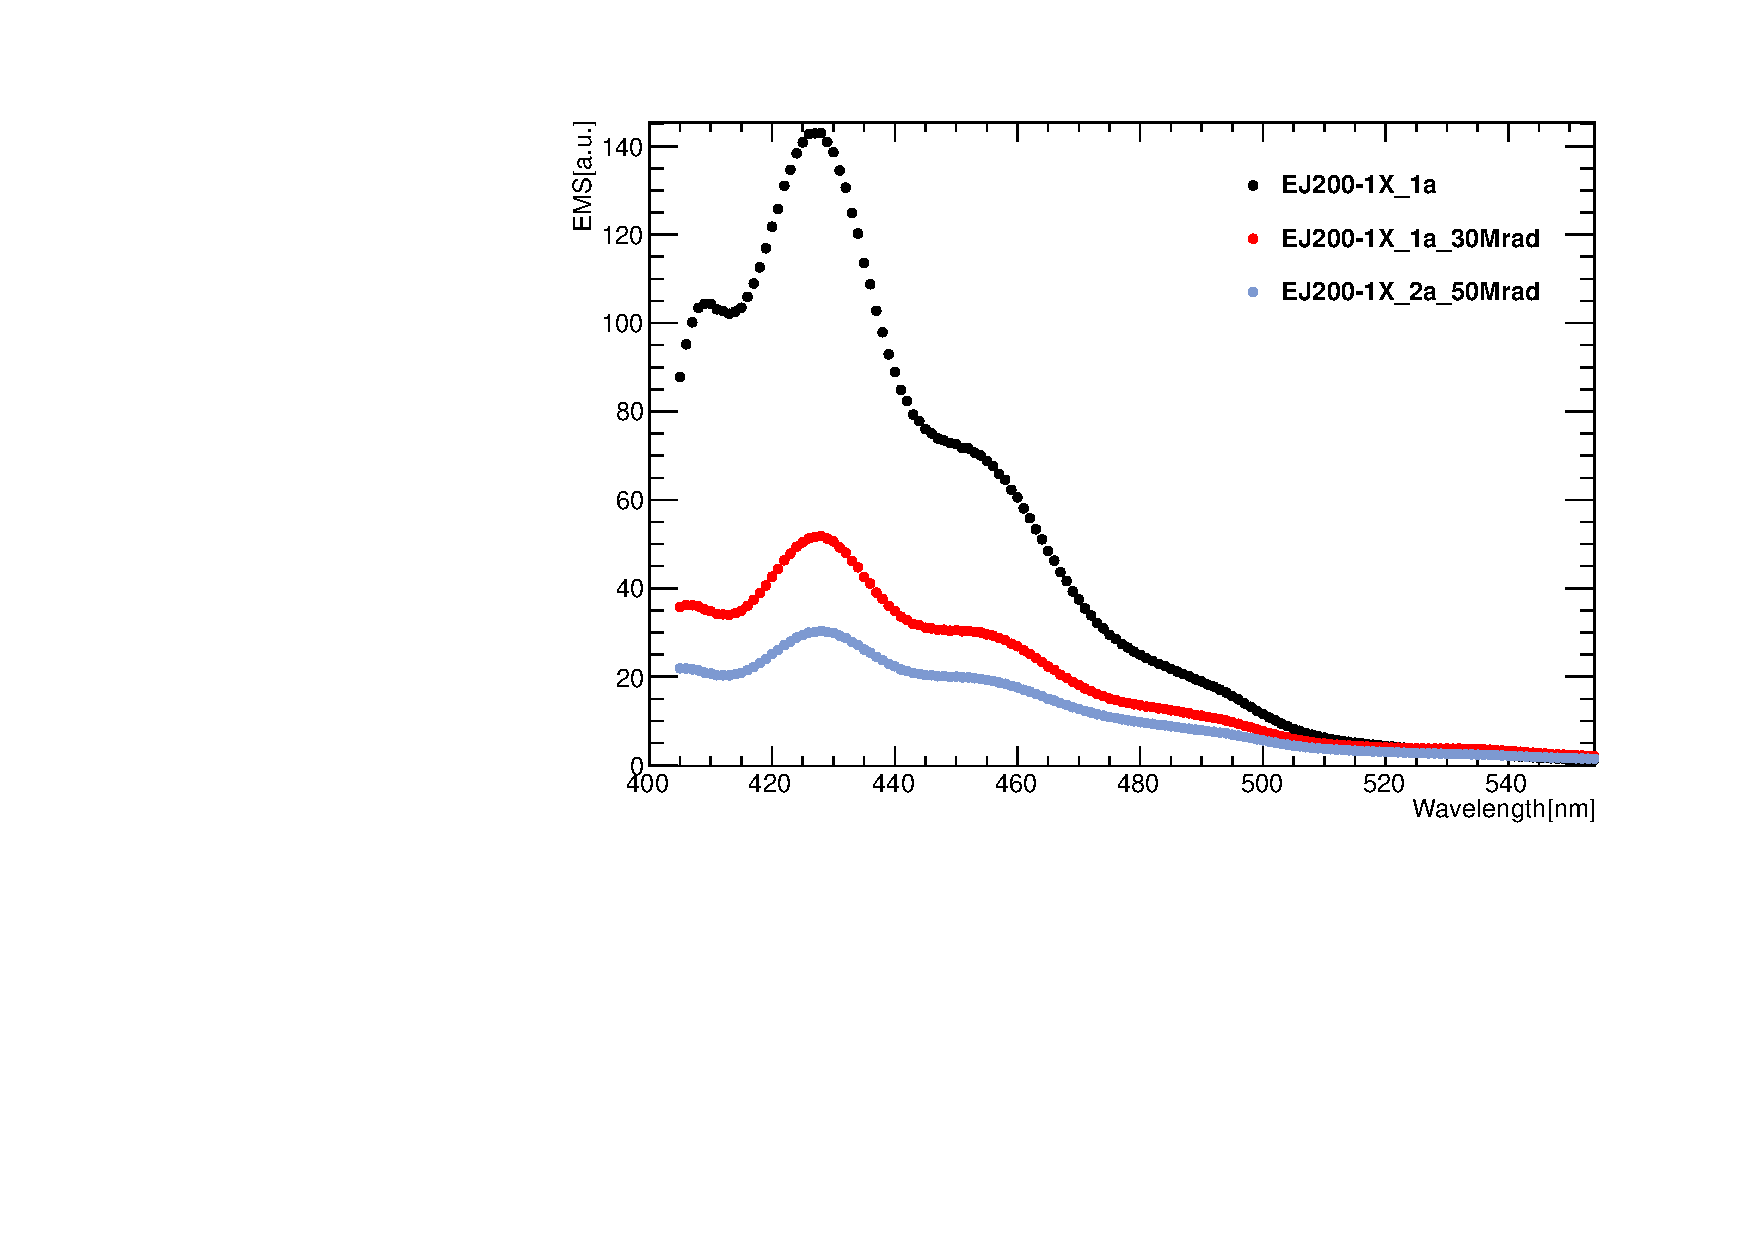
\includegraphics[width=0.49\textwidth]{plot_EJ200-1X_EMS.pdf}
\caption{
Emission spectrum for EJ-408 at nominal doping before irradiation, after 30 Mrad at 1 Mrad/hr and after 50 Mrad at 1 Mrad/hr.
}
\label{fig:ej408doping1x}
\end{center}
\end{figure}


\section{Interpretation}


If this dose rate effect is due to oxygen diffusion, then
we expect it to be governed by the diffusion equation.  Since
the oxygen diffusion depth is greater at lower dose rates,
we expect the damage for the same dose at different dose rates to
increase up to the point where the dose rate is low enough that oxygen
permeates the entire sample.  The dose rate effect should plateau
at this point.  Specifically, we predict that the light output
reduction should depend on both the dose and the dose rate as:
$$ L(R,D) = 1 - [f(D)Z(R) + a(D)(1-Z(R))]$$
where L is the \% light yield, D is the dose, R is the dose rate, 
Z(R) is the fraction of the scintillator containing 
oxygen and is given by $min({{2 z_0(R)}\over{d}},1)$
where d is the thickness of the scintillator and $z_0$ gives
the depth of scintillator penetrated by oxygen,
a(D) is related to the fraction of quenching in the part of
the scintillator containing oxygen and is given by $1-e^{-a_0 D}$, 
and
f(D) is related to the fraction of quenching in the part of
the scintillator not containing oxygen and is given by $1-e^{-f_0 D}$.
The diffusion depth $z_0(R)$ is given by diffusion theory as 
$$z_0(R)=\sqrt{\gamma/R}$$
where $\gamma$ is a property of the substrate and the radicals that
are dissolved in that substrate during the diffusion process.
The value for $\gamma$ depends on the material, oxygen pressure,
radical concentration (which is proportional to the dose) and 
temperature.
The minimization in Z(R) occurs because the fraction of scintillator
containing oxygen can not exceed one.  Note that this equation 
assumes the temperature and the surrounding atmosphere
is held constant, as this can 
affect diffusion.


\section{Conclusions}

\section{Acknowledgements}
The authors would like to thank Neil Blough and Anna Pla-Dalmau for advice on taking fluorescence measurements, and Blough for the use of his machine.  This work was supported in part by U.S. Department of Energy Grant YYYYY.

\section*{References}

\bibliography{afluorescence}

\end{document}